\documentclass[12pt,twoside]{report}
\usepackage[T1]{fontenc}
\usepackage{longtable}
\usepackage[utf8]{inputenc}
\usepackage{multicol}
\usepackage{amsmath}
\usepackage{gensymb}
\setlength{\columnsep}{1cm}
\usepackage{graphicx}
\usepackage{newtxtext,newtxmath}
\graphicspath{{figures/}}
\setcounter{tocdepth}{5}
\usepackage{caption}
\usepackage{subfig}
\usepackage{hyperref}
\usepackage{setspace}
\usepackage{pdfpages}
\usepackage[style=ieee,
            hyperref=true,
            url=false,
            date=year,
            isbn=false,
            backref=false,
            doi=false,
            citereset=chapter,
            block=none]{biblatex}
\addbibresource{references.bib}
\usepackage{enumitem,lipsum}
\usepackage{titlesec}
\usepackage{nopageno}
\titleformat{\chapter}[display]
  {\normalfont\bfseries}{}{0pt}{\Large}
\usepackage{geometry}
 \geometry{
 a4paper,
 lmargin=0.8in,
 tmargin=1in,
 bmargin=1in,
 rmargin=0.8in
 }
\usepackage{fancyhdr}
\usepackage[utf8]{inputenc}
\pagestyle{fancy}
\fancyhf{}
\fancyhead[RE]{\leftmark}
\fancyhead[LO]{\rightmark}
\fancyfoot[RO,LE]{\thepage}
\fancypagestyle{plain}{
\renewcommand\headrulewidth{0pt}
\fancyhf{}
\fancyfoot[R]{\thepage}
}
\pagenumbering{roman}
\newcommand{\thesistitle}{\MakeUppercase{IOT Based 3 Phase Induction Motor control and monitoring
}} 
\title{\thesistitle}
\begin{document}
\begin{titlepage}
    \begin{center}
        \textsc{\textbf{\Large{\thesistitle}}}
        
        \vspace{1.5cm}
        \textit{\large{Drives, Controls and Modelling Lab Mini Project}}\\
        
        
        \vspace{10cm}
        \textit{\large{Submitted by}}
        \vspace{1cm}
        \begin{flushleft}
        \begin{multicols}{2}
            \textsc{Mohammed Aman Kanjirathinkal Sunil}\\
            \textsc{John Biju}\\
            \textsc{Adithya Pradosh}
            
            \columnbreak
            \textsc{190929023, Section A - Mechatronics}\\
            \textsc{190929013, Section A - Mechatronics}\\
            \textsc{190929108, Section A - Mechatronics}
        \end{multicols}
        \end{flushleft}
        
        \vspace{3cm}
        {
\includegraphics[height=0.09\textheight, width=1\textwidth]{Figures/mit.jpg}}
        
        \vspace{0.5cm}
        \textbf{30 November, 2020}
        
    \end{center}
\end{titlepage}
\titleformat{\chapter}[display]{\bfseries\centering}{\large}{1em}{\large}
\newpage

\chapter{INTRODUCTION}
\setcounter{page}{1}
\pagenumbering{arabic}
Induction Motor is a singly-excited device that works on the principle of Mutual Induction. It is similar to a transformer which also works on the same principle. The difference between a transformer and IM is the transformer is a static device, whereas the IM is a rotating device. In industry, 90% of use the induction motor because of necessary characteristics. It is an inherent self-start motor, and it does not require a permanent magnet, No brushes, No commutator rings, No position sensor. The induction motor also has a simple and robust operation, maintains a good power factor, less maintenance, is highly efficient, small in size, reliable, and cheaper than other types of motor.
This project deals with the hardware for monitoring the continuous parameters and speed control part of the Induction Motor. With the help of sensors, monitored parameters are a voltage sensor, current sensor, speed sensor.

\section{Objectives}
\begin{itemize}
    \item {For safe and economic data communication in industry or any other field, monitoring and controlling the operation of an induction motor depend on the internet of Things (IoT) is to do.}
    \item {By early fault detection, process interruption of the motor can be reduced, reducing damages of the motor in an industrial process to a more significant extent, which makes the motor more reliable.}
    \item {To protect the motor from overloading, over-current, and high temperature.}
\end{itemize}

\section{Faults}
In Induction Motor number of types of faults that occur widely, it is subdivided into three most important parts such as 
\begin{itemize}
    \item {Electrical faults: In electrical fault commonly occurs a single phasing fault, Reverse phase sequencing fault, oversupply voltage, overload fault, Earth fault, etc.}
    \item {Mechanical Faults: In mechanical fault usually occurs a rotor broken bar fault, stator and rotor winding defect, Bearing fault, etc.}
    \item {Environment Faults: In an environment, fault typically occurs the vibration of the motor, Induction Motor surrounding environment affects the performance of an Induction Motor such as moisture, temperature, etc.}
\end{itemize}

\section{Brief Importance}
Dynamic motor testing is quickly becoming a crucial part of all good predictive maintenance programs as innovations continue to evolve in software and hardware upgrades. Monitoring supports the reliability engineer's approach to maintaining a safe, effective, and productive operation. Monitoring motor performance with adequately trained technicians using modern equipment allows plant managers to dictate their downtime, improve plant operations, and quickly identify poorly performing equipment. Monitoring motors' performance and making necessary adjustments will improve reliability, extend the motor's life, and reduce the facility's overall operating cost.
This project is about IoT-based Induction Motor monitoring parameters such as voltage, current, speed based on the sensor. The speed of the induction motor is controlled with the help of the PWM technique, as its speed can be controlled easily by controlling the input power of frequency. Continuous monitoring of the parameters maintains the continuity of production in industries, making the motor reliable, i.e., the production of an industry can be increased. Also, it prevents any abnormality in the induction motor and detects the early fault in the induction motor. 
Suppose there is any fault that takes place in the motor. In that case, it will be determined by a sensor that senses the parameter values of voltage, current, speed, and the respective output values by the sensor give a signal to Arduino Uno, which sends a command to the computer that the motor should automatically be disconnected from the system.


\chapter{MATERIALS AND METHODOLOGY}
\section{Software Requirements}
\begin{itemize}
    \item {MATLAB}
    \item {Simulink}
\end{itemize}

\section{Hardware Requirements}
Following are the required components:
\begin{itemize}
    \item {Induction motor.}
    \item {Arduino UNO.}
    \item {Condition monitoring Sensors (Like Voltage transformer, Current transformer, Speed sensor)}
    \item {Speed controlling Device.}
    \item {Gate Driver Circuit.}
    \item {LCD}
    \item {ESP8266(WIFI Module).}
\end{itemize}

\section{Induction Motor}
The induction motor is known as an asynchronous motor. The induction motor has its advantages like its necessary characteristic, robustness, and effectiveness than any other type of Motor. Here in our project, induction motor plays a significant role.\\
Parameters:\\
Volts-415v \\
Frequency- 50Hz\\
Speed- 1440 rpm\\
{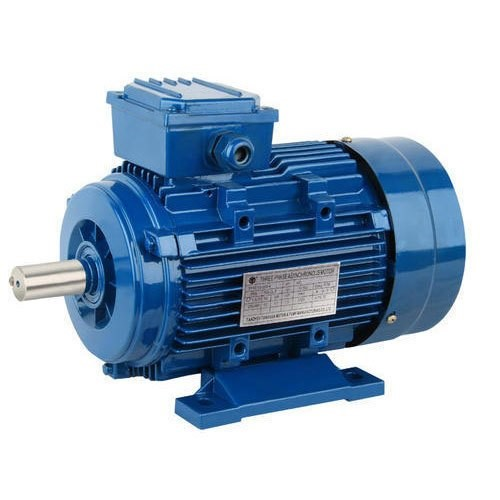
\includegraphics[height=0.2\textheight]{Figures/motor.jpg}}

\section{Arduino UNO}
Arduino Uno is a low-cost, flexible, and easy-to-use programmable open-source microcontroller board that can be integrated into various electronic projects. This board can be interfaced with other Arduino boards, Arduino shields, Raspberry Pi boards and can control relays, LEDs, servos, and motors as an output.\\
{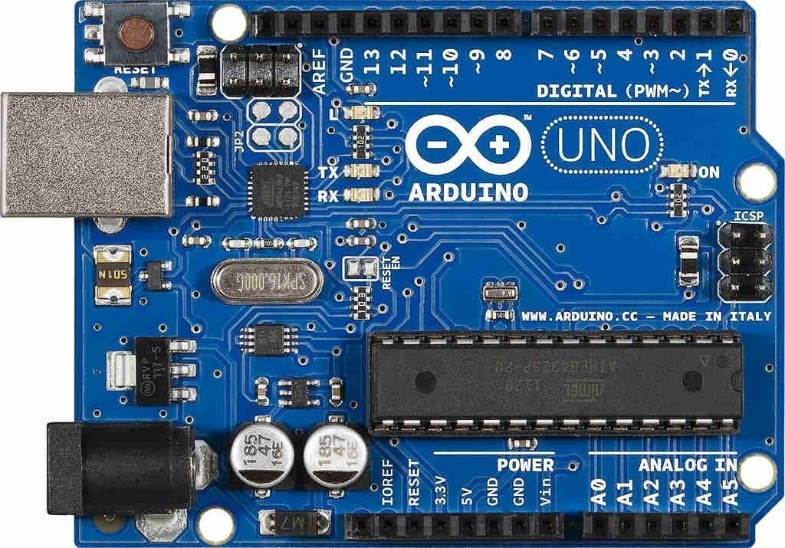
\includegraphics[height=0.2\textheight]{Figures/arduino.jpg}}

\section{Conditional Monitoring Sensor}
There are three sensors used for monitoring and evaluation management in the system.\\
\begin{itemize}
    \item {We use a voltage transformer to measure the supply voltage as it acts as a step-down and sensing of the supply voltage.}
    \item {Current transformer for measuring motor current}
    \item {IR Sensor for measuring speed}
\end{itemize}
\subsection{Voltage Transformer}
The voltage transformer is used for measuring high alternating voltage purposes; here in this project, it also acts as a sensor for sensing the supply voltage of an Induction Motor. It is a step-down transformer that converts 230 v to 4 v supply.\\
{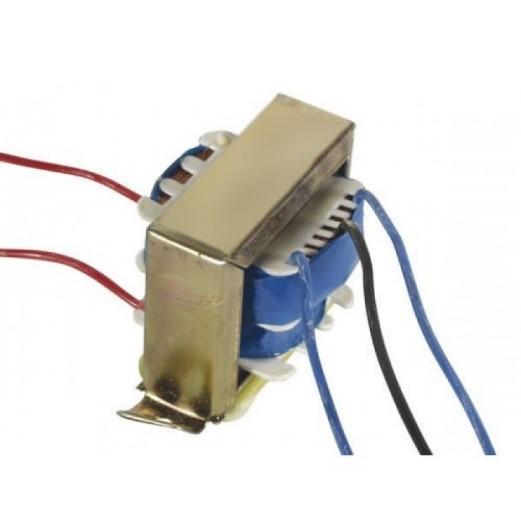
\includegraphics[height=0.2\textheight]{Figures/volt.jpg}}
\section{Current Transformer}
The current transformer is used to measure high alternating current, and here it also acts as a sensor for sensing the current that flows in the Induction Motor. It has an input current rating of 5A, and an analogy output current rating is 5mA. It is a 5A range of single-phase AC sensor modules. It has a 1000: 1 turn ratio.\\
{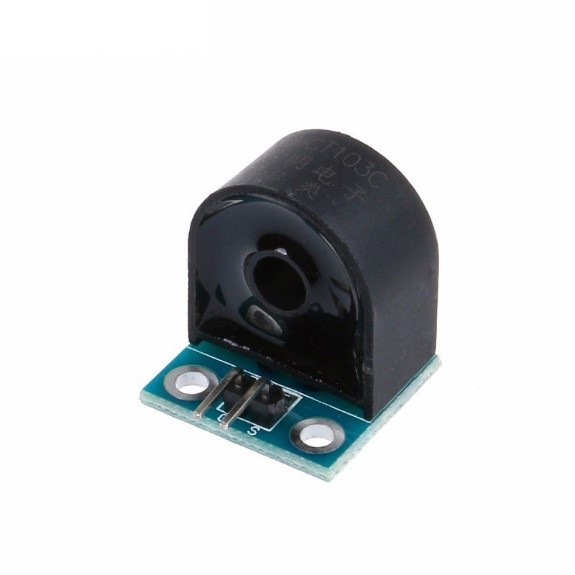
\includegraphics[height=0.2\textheight]{Figures/trans.jpg}}
\subsection{IR Sensor Module}
It is an electronic device to measure and detect infrared radiation from its surrounding atmosphere. It includes LED and an infrared laser diode. It works as a digital tachometer. IR sensor used for measuring the speed of 3 phase Induction Motor in rpm. It has an operating voltage that is 3 to 5v.\\
{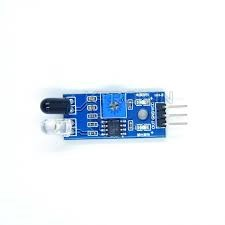
\includegraphics[height=0.2\textheight]{Figures/ir.jpg}}
\subsection{Speed Controlling Device}
BT139 Triac is a semiconductor device with a plastic envelope packaged, high bidirectional transistor, and high blocking voltage capability. BT139 is a Triac switch used for the speed controlling purpose of an induction motor with the help of the gate triggering circuit. The gate driver circuit is for logical purposes to operate the Triac switch.\\
{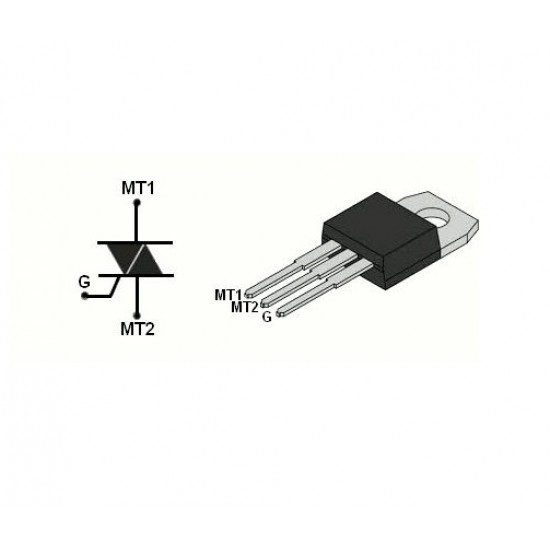
\includegraphics[height=0.2\textheight]{Figures/triac.jpg}}
\subsection{LCD Display}
LCD is an electronic screen display module. The type of LCD used in this proposed system for continuously displaying the monitored value of an induction motor is 16x4. Here 16 values indicate the character on a single line, and four indicate the number of lines. Operation of LCD requires a 5V DC supply.\\
{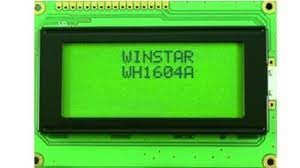
\includegraphics[height=0.2\textheight]{Figures/lcd.jpg}}
\subsection{ESP8266}
We use the Wi-Fi module for communication with the cloud. We have used the ESP8266 Wi-Fi module to exchange information between devices to the cloud without connecting to any wire. Each device has its I.P address. For connection to the cloud,  the I.P address is entered on the Android application, and the devices in the system, i.e., induction motor, sensors, speed controlling device. 
These are connected to the cloud and send information to the cloud without any wired connection, i.e., through the Wi-Fi module send information for further process.
{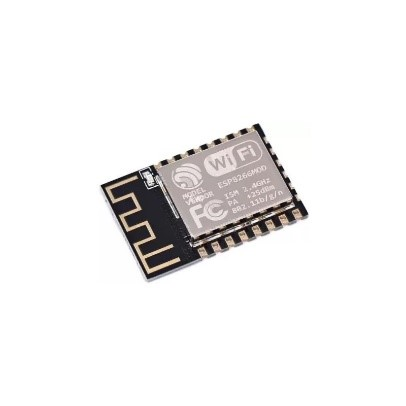
\includegraphics[height=0.2\textheight]{Figures/esp.jpg}}

\section{Block Diagram}
{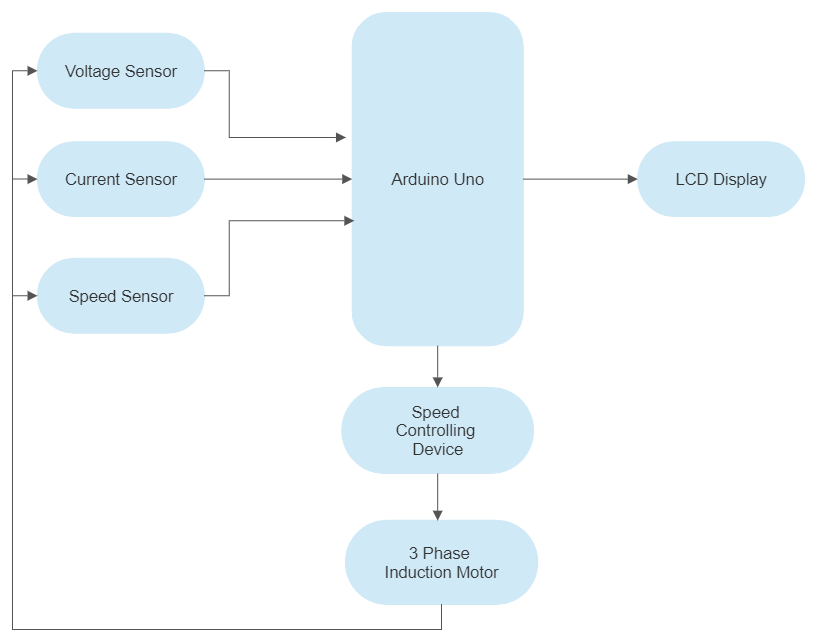
\includegraphics[height=0.5\textheight]{Figures/Drawing.jpg}}

\section{Method}
3 phase AC supply comes into the system; from AC supply to 3 phase Induction Motor through a speed controlling device and gate driver circuit. Here, the gate driver circuit acts as a logic circuit to on-off the switches to control the motor's speed. There are many methods to control the speed of the motor, but the PWM technique has been used here to control the speed of an induction motor. PWM technique is very sophisticated to use and most sophisticated to operate than any other method. By adjusting the ON-OFF period of TRIAC switches controlling the firing angle and, from that, the firing angle controls the speed of the induction motor.






\chapter{RESULTS}
AC voltage of frequency 50hz is fed to the induction motor by converting a DC voltage of 100V and resistive load of 10ohm using a DC-AC inverter.\\ 
The speed of the motor is then controlled by using Pulse Width Modulation techique using a gate driver circuit consisting TRIAC switches. The ON-OFF period of the TRIAC switches are adjusted by signals from the Arduino UNO unit.\\ 
The Arduino UNO unit is provided a 5V DC current provided by a step down transformer with a rectifier and a regulator.\\ 
The speed of the motor is measured with a tachometer and compared with the frequency of the PWM signal generated.\\
{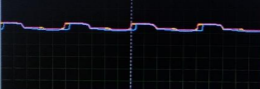
\includegraphics[height=0.18\textheight]{Figures/g1.png}}
\\
{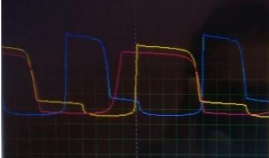
\includegraphics[height=0.2\textheight]{Figures/g2.png}}
\\
Generated PWM signal
\\
{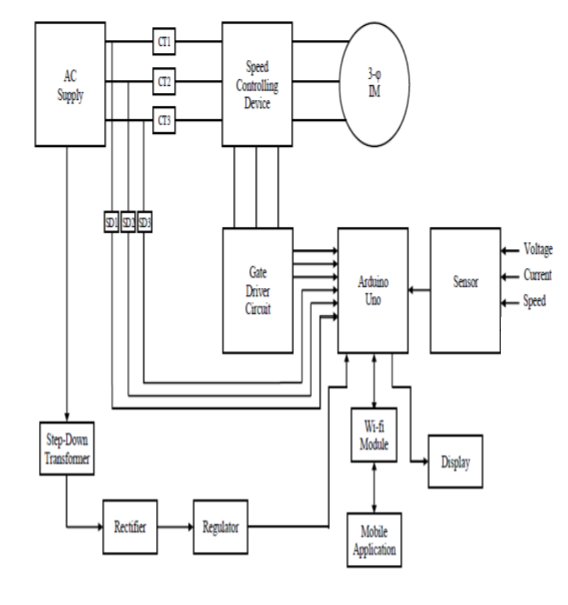
\includegraphics[height=0.4\textheight]{Figures/g3.png}}
\\
The above block diagram shows the detailed view of the project. It describes the whole project in one single diagram.
\\ \\
{\large Simulation}
\\ \\
{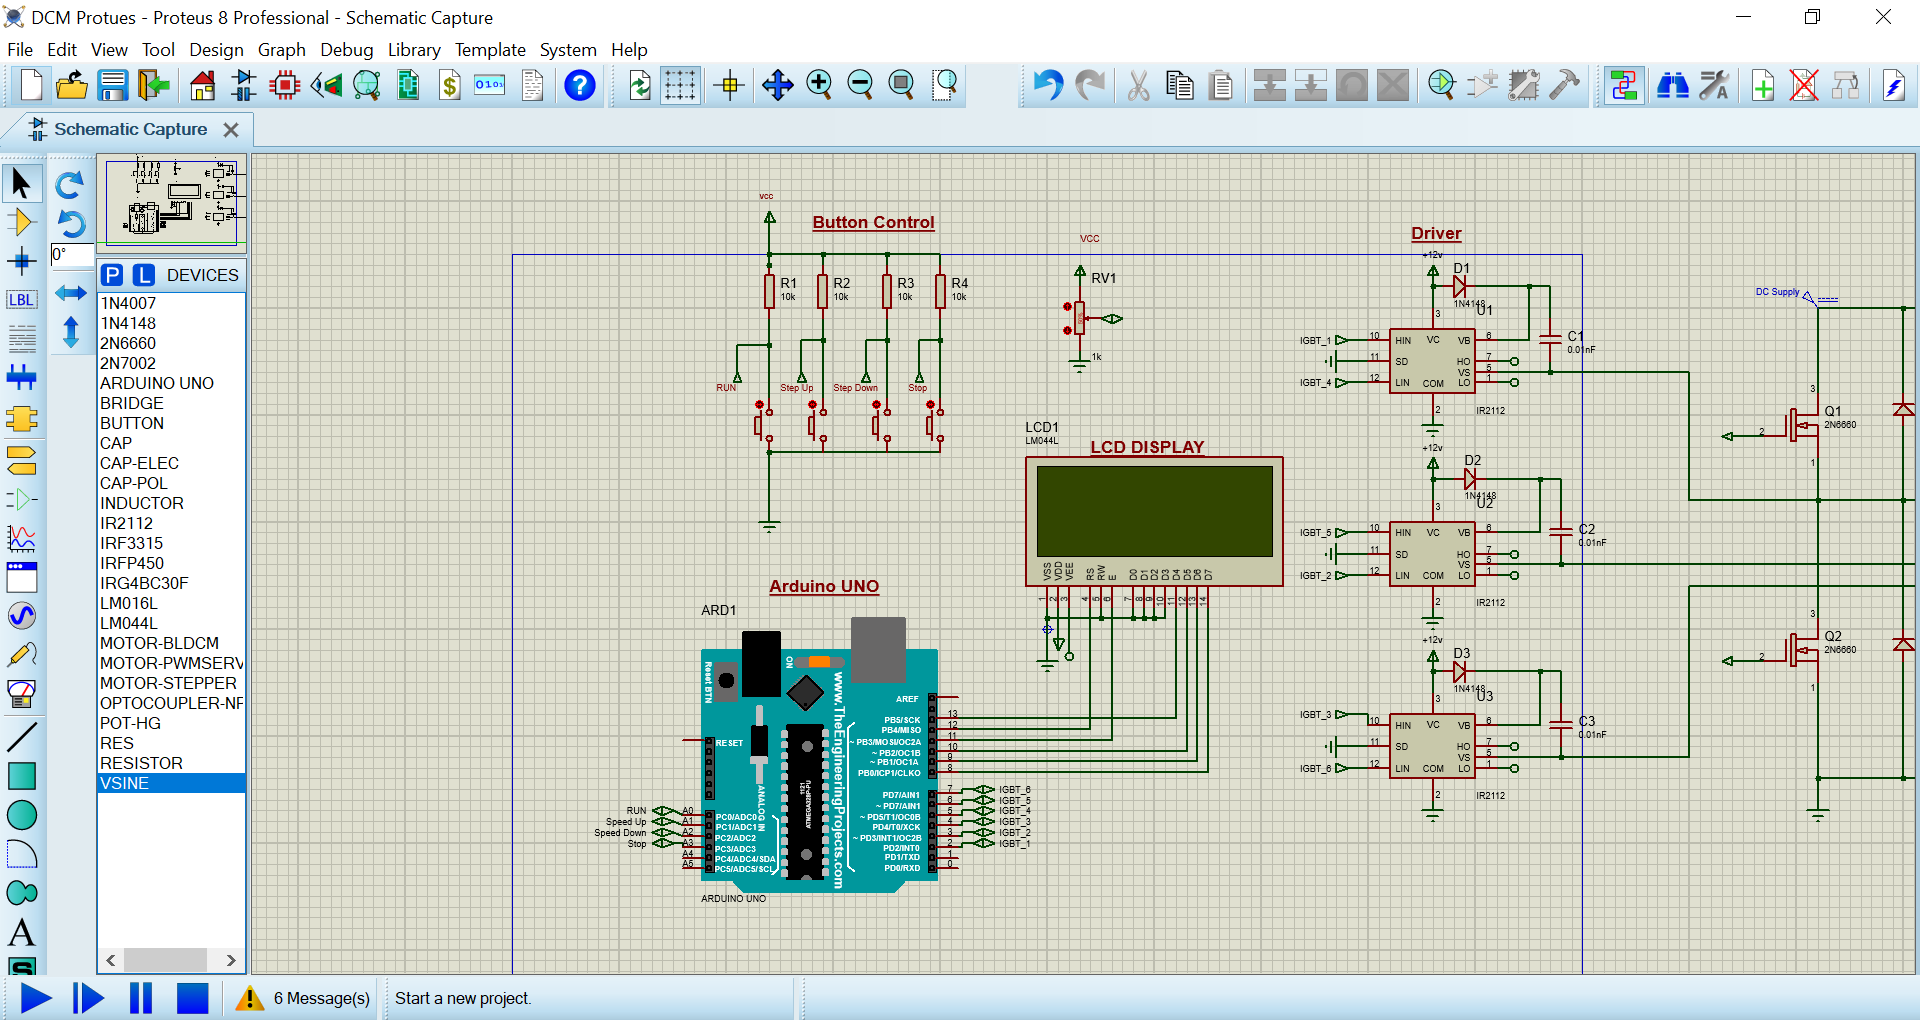
\includegraphics[height=0.3\textheight]{Figures/pro1.png}}
\\
{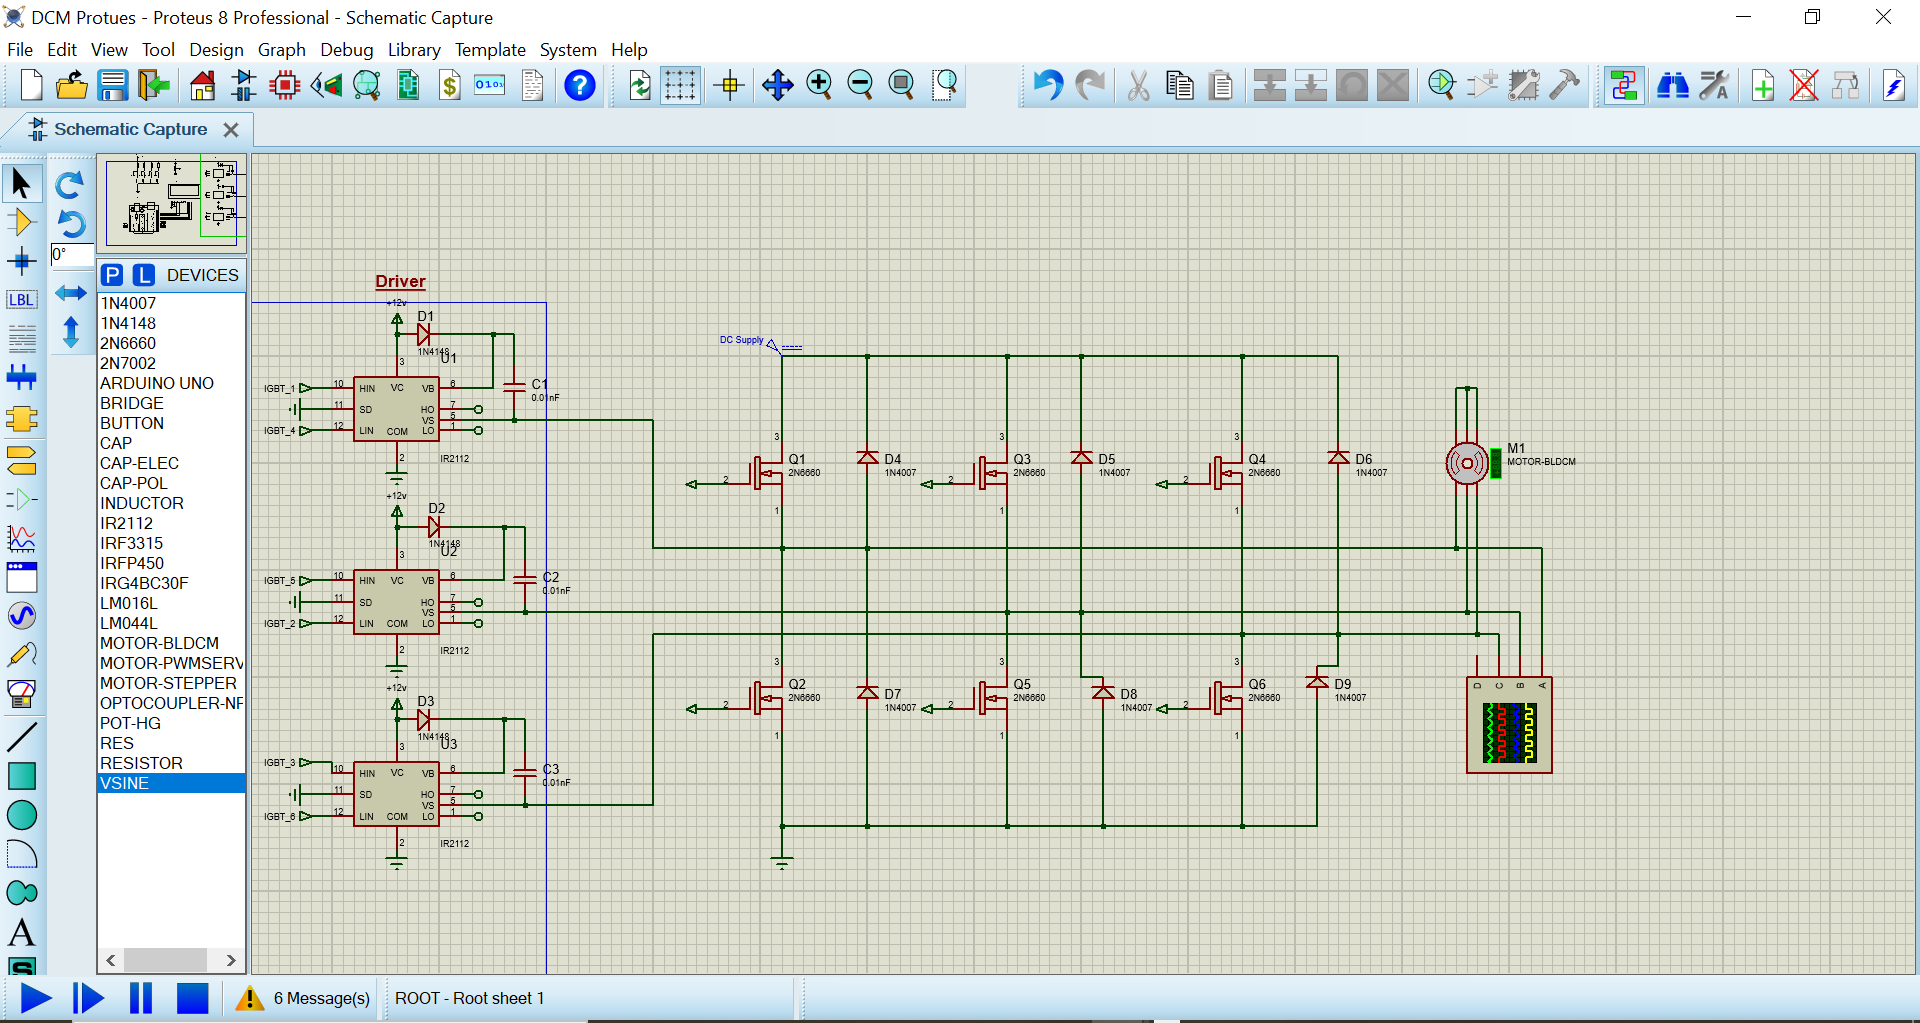
\includegraphics[height=0.3\textheight]{Figures/pro2.png}}
\\ \\







\chapter{CONCLUSION AND SCOPE OF FUTURE WORK}
This project represents the impact of IoT is well known and is a rapidly growing technology. Now IoT has become a vital part of human life. Recently IoT has come all over the field such as industry, home automation, electric vehicle, traction, agriculture, medical field, etc., with the help of sensors. This project represents IoT-based condition monitoring parameters and controlling the speed of the motor with the help of the PWM technique. By analyzing the motor parameters, make the motor-operated safe and protective. It also helps in calculating new data to interact with social media and others. In industries require continuous monitoring of data value for power consumption and maintenance applications. If the motor gets over current, speed, and excessive temperature than its rated value, it will automatically disconnect from the supply.\\
\end{document}